\section{Durchführung}
\label{sec:Durchführung}

\subsection{(a) Erzeugen einer amplitudenmodulierten Schwingung mit
Hilfe eines Ringmodulators(keine Trägerabstrahlung)}
\label{subsec:durchfuehrung_a}
Zur Amplitudenmodulation durch einen Ringmodulator wir ein Aufbau,
entsprechend des Schaltbildes in Abbildung \ref{fig:schaltung_a}, verwendet.
Anschließend wird ein Bild, das Modulationssignal sowie moduliertes
Signal im Zeitraum zeigt, am Oszillographen aufgenommen.

\begin{figure}
  \centering
  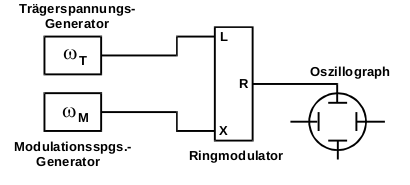
\includegraphics[width=0.7\textwidth]{figures/a_d.png}
  \caption{Verwendete Schaltung zur Amplitudenmodulation mit Ringmodulator.\cite{sample}}
  \label{fig:schaltung_a}
\end{figure}


\subsection{(b) Untersuchung des Frequenzspektrums einer
amplitudenmodulierten Schwingung}
\label{subsec:durchfuehrung_b}
Um das Frequenzspektrum des in Abschnitt \ref{subsec:durchfuehrung_a} generierten
amplitudenmodulierten Signals zu untersuchen, wird in Abbildung
\ref{fig:schaltung_a} der Oszillograph durch einen Frequenzanalysator ersetzt.
Es wird ein Bild des Frequenzspektrums zwischen $\SI{324}{\hertz}$ und $\SI{1424}{\hertz}$
aufgenommen.


\subsection{(c) Erzeugen einer amplitudenmodulierten Schwingung
mit Hilfe einer Gleichrichterdiode (inklusive Trägerabstrahlung)}
\label{subsec:durchfuehrung_c}
Mit Hilfe der in Abbildung \ref{fig:schaltung_c} gezeigten Schaltung,
wird ein amplitudenmoduliertes Signal mit Trägerfrequenzabstrahlung erzeugt.
Das generierte Signal wird sowohl im Zeitbereich am Oszilloskop, als auch
im Frequenzbereich am Frequenzanalysator, dargestellt.

\begin{figure}
  \centering
  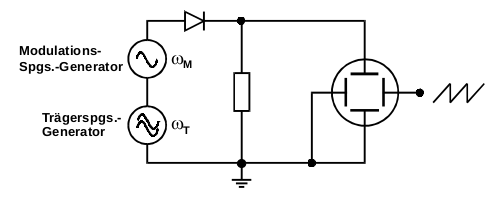
\includegraphics[width=0.7\textwidth]{figures/c_d.png}
  \caption{Verwendete Schaltung zur Amplitudenmodulation mit Diode.\cite{sample}}
  \label{fig:schaltung_c}
\end{figure}


\subsection{(d) Erzeugen einer frequenzmodulierten Schwingung}
\label{subsec:durchfuehrung_d}


\subsection{(e) Untersuchung der Phasenabhängigkeit eines
phasenempfindlichen Gleichrichters}
\label{subsec:durchfuehrung_e}


\subsection{(f) Demodulation einer amplitudenmodulierten Schwingung
mit Hilfe eines Ringmodulators}
\label{subsec:durchfuehrung_f}


\subsection{(g) Demodulation einer amplitudenmodulierten Schwingung
mit Hilfe einer Gleichrichterdiode}
\label{subsec:durchfuehrung_g}


\subsection{(h) Demoduolation einer frequenzmodulierten Schwingung
mit Hilfe eines Flankendemodulators}
\label{subsec:durchfuehrung_h}
